\documentclass[crop,tikz]{standalone}
	\usetikzlibrary{patterns}
\begin{document}
	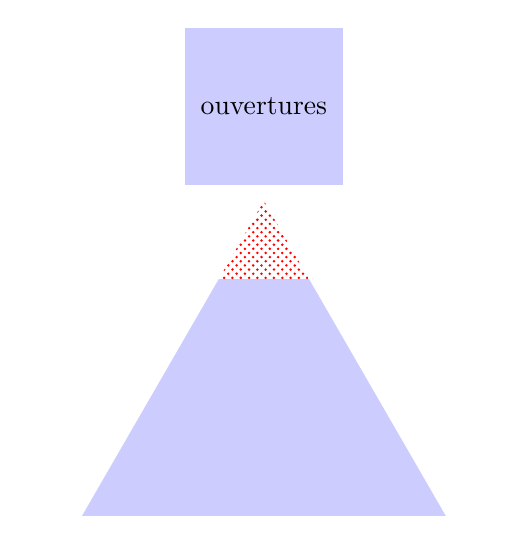
\begin{tikzpicture}
		\fill[color=blue!20] (-1, 3.2) rectangle (1,5.2) node[color=black,pos=.5] {ouvertures};
 		\begin{scope}
	 		\clip (-3,-1) rectangle (3,2);
	 		\fill[color=blue!20] (90:3cm) \foreach \x in {210,330} {
	 			-- (\x:3cm)
	 		} -- cycle (60:3cm) ;
 		\end{scope}
 		\begin{scope}
			\clip (-1,2) rectangle (1,3);
			\fill[pattern=crosshatch dots, pattern color=red] (90:3cm) \foreach \x in {210,330} {
				-- (\x:3cm)
			} -- cycle (60:3cm) ;
 		\end{scope}
	\end{tikzpicture}
\end{document}